%%% Title presen0614
\documentclass[landscape,10pt]{ujarticle}
\special{papersize=\the\paperwidth,\the\paperheight}
\usepackage{ketpic,ketlayer}
\usepackage{ketslide}
\usepackage{amsmath,amssymb}
\usepackage{bm,enumerate}
\usepackage[dvipdfmx]{graphicx}
\usepackage{color}
\definecolor{slidecolora}{cmyk}{0.98,0.13,0,0.43}
\definecolor{slidecolorb}{cmyk}{0.2,0,0,0}
\definecolor{slidecolorc}{cmyk}{0.2,0,0,0}
\definecolor{slidecolord}{cmyk}{0.2,0,0,0}
\definecolor{slidecolore}{cmyk}{0,0,0,0.5}
\definecolor{slidecolorf}{cmyk}{0,0,0,0.5}
\definecolor{slidecolori}{cmyk}{0.98,0.13,0,0.43}
\def\setthin#1{\def\thin{#1}}
\setthin{0}
\newcommand{\slidepage}[1][s]{%
\setcounter{ketpicctra}{18}%
\if#1m \setcounter{ketpicctra}{1}\fi
\hypersetup{linkcolor=black}%

\begin{layer}{118}{0}
\putnotee{122}{-\theketpicctra.05}{\small\thepage/\pageref{pageend}}
\end{layer}\hypersetup{linkcolor=blue}

}
\usepackage{emath}
\usepackage{emathEy}
\usepackage{emathMw}
\usepackage{pict2e}
\usepackage{ketlayermorewith2e}
\usepackage[dvipdfmx,colorlinks=true,linkcolor=blue,filecolor=blue]{hyperref}
\newcommand{\hiduke}{0614}
\newcommand{\hako}[2][1]{\fbox{\raisebox{#1mm}{\mbox{}}\raisebox{-#1mm}{\mbox{}}\,\phantom{#2}\,}}
\newcommand{\hakoa}[2][1]{\fbox{\raisebox{#1mm}{\mbox{}}\raisebox{-#1mm}{\mbox{}}\,#2\,}}
\newcommand{\hakom}[2][1]{\hako[#1]{$#2$}}
\newcommand{\hakoma}[2][1]{\hakoa[#1]{$#2$}}
\def\rad{\;\mathrm{rad}}
\def\deg#1{#1^{\circ}}
\newcommand{\sbunsuu}[2]{\scalebox{0.6}{$\bunsuu{#1}{#2}$}}
\def\pow{$\hspace{-1.5mm}^\hspace{-1mm}$}
\def\dlim{\displaystyle\lim}
\newcommand{\brd}[2][1]{\scalebox{#1}{\color{red}\fbox{\color{black}$#2$}}}
\newcommand\down[1][0.5zw]{\vspace{#1}\\}
\newcommand{\sfrac}[3][0.65]{\scalebox{#1}{$\frac{#2}{#3}$}}
\newcommand{\phn}[1]{\phantom{#1}}
\newcommand{\scb}[2][0.6]{\scalebox{#1}{#2}}
\newcommand{\dsum}{\displaystyle\sum}

\setmargin{25}{145}{15}{100}

\ketslideinit

\pagestyle{empty}

\begin{document}

\begin{layer}{120}{0}
\putnotese{0}{0}{{\Large\bf
\color[cmyk]{1,1,0,0}

\begin{layer}{120}{0}
{\Huge \putnotes{60}{20}{インストール状況}}
\putnotes{60}{50}{高遠節夫}
\end{layer}

}
}
\end{layer}

\def\mainslidetitley{22}
\def\ketcletter{slidecolora}
\def\ketcbox{slidecolorb}
\def\ketdbox{slidecolorc}
\def\ketcframe{slidecolord}
\def\ketcshadow{slidecolore}
\def\ketdshadow{slidecolorf}
\def\slidetitlex{6}
\def\slidetitlesize{1.3}
\def\mketcletter{slidecolori}
\def\mketcbox{yellow}
\def\mketdbox{yellow}
\def\mketcframe{yellow}
\def\mslidetitlex{62}
\def\mslidetitlesize{2}

\color{black}
\Large\bf\boldmath
\addtocounter{page}{-1}

\def\MARU{}
\renewcommand{\MARU}[1]{{\ooalign{\hfil$#1$\/\hfil\crcr\raise.167ex\hbox{\mathhexbox20D}}}}
\renewcommand{\slidepage}[1][s]{%
\setcounter{ketpicctra}{18}%
\if#1m \setcounter{ketpicctra}{1}\fi
\hypersetup{linkcolor=black}%
\begin{layer}{118}{0}
\putnotee{115}{-\theketpicctra.05}{\small\hiduke-\thepage/\pageref{pageend}}
\end{layer}\hypersetup{linkcolor=blue}
}
\newcounter{ban}
\setcounter{ban}{1}
\newcommand{\monban}[1][\hiduke]{%
#1-\theban\ %
\addtocounter{ban}{1}%
}
\newcommand{\monbannoadd}[1][\hiduke]{%
#1-\theban\ %
}
\newcommand{\addban}{%
\addtocounter{ban}{1}%%210614
}
\newcounter{edawidth}
\newcounter{edactr}
\newcommand{\seteda}[1]{
\setcounter{edawidth}{#1}
\setcounter{edactr}{1}
}
\newcommand{\eda}[2][\theedawidth ]{%
\noindent\Ltab{#1 mm}{[\theedactr]\ #2}%
\addtocounter{edactr}{1}%
}
%%%%%%%%%%%%

%%%%%%%%%%%%%%%%%%%%

\newslide{GCの利用}

\vspace*{18mm}

\slidepage
\begin{itemize}
\item
課題のやり取りをGC(GoogleClassroom)で行う.
\item
課題は,htmlの形で配付する.
\item
課題の Pgの下にある矢印を押してページを変える\\
 ・{\color{red}「Q---」はタイトルページなので入力しない}
\item
[課題]\monban 出席と準備状況を聞きます.\seteda{60}\\
\eda{出席していたら「はい」,そうでなければ「いいえ」}\\
\eda{KeTCindyの動作確認ができているか}
\end{itemize}
%%%%%%%%%%%%

%%%%%%%%%%%%%%%%%%%%


\newslide{KeTCindyによる作図手順}

\vspace*{18mm}

\slidepage
\begin{enumerate}[1.]
\item
ユーザホームのketcindy(+日付)フォルダを開く
\item
temlate(samples)の1つのcdyファイルをクリック\\
 ・例えば,01figure.cdyを用いる\\
 ・Cinderellaを直接立ち上げない\\
 ・他のフォルダに移したり名前を変えてもいい\\
 ・名前には全角文字や半角スペースを使わない
\item
トップメニューから「スクリプト」>Scriptを開く\\
\end{enumerate}

\newslide{KeTCindyによる作図手順(続)}

\vspace*{18mm}

\slidepage
\begin{enumerate}[1.]
\setcounter{enumi}{3}
\item
適宜Cindy画面に点(幾何点)を追加する\\
 ・幾何点は画面で移動できる\\
 ・Scriptで点(リスト点)を追加することもできる\\
    p1=[3,2]; (動かすには座標を変更)
\item
KetinitからWindispgの間のスクリプトを修正する
\item
右上のギヤマークを押すとCindy画面の図が変わる
\item
Figureボタンを押すとTeXが走ってPDFができる
\end{enumerate}

\newslide{幾何点とリスト点}

\vspace*{18mm}

\slidepage
\begin{itemize}
\item
templatesの01figure.cdyを開く
\item
画面の幾何点Cを消去する\\
 ・点をクリックして「消しゴム」ツール
\item
Scriptを見るとコンソールにエラーが出ている\\
 ・3行目のコマンドでCがないから
\item
リスト点pCを追加する\\
 ・pC=[ ];
A,B,pCの三角形をかく
\end{itemize}

\newslide{課題(幾何点とリスト点)}

\vspace*{18mm}

\slidepage
\begin{itemize}
\item
[課題]\monban 以下に答えよ\seteda{60}\\
\eda{pC=...の行をコピペせよ}\\
\eda{A,B,pCの三角形をかく行をコピペせよ}
\end{itemize}
%%%%%%%%%%%%

%%%%%%%%%%%%%%%%%%%%


\newslide{KeTCindyのヘルプ}

\vspace*{18mm}

\slidepage
\begin{itemize}
\item
KeTCindyのリファレンス\\
 ・ユーザホームのKeTCindyReferenceJ.pdf\vspace{-1mm}
\item
Cinderellaのヘルプ\\
 ・トップメニューのヘルプからマニュアルをクリック\vspace{-1mm}
\item
KeTCindyのコマンドは大文字から始まる\vspace{-1mm}
\item
スクリプト画面(の最後)に Help("Listplot");\\
・簡単な説明(例)が表示される\\
・大文字小文字を区別する
\end{itemize}
%%%%%%%%%%%%

%%%%%%%%%%%%%%%%%%%%


\newslide{関数のグラフPlotdata}

\vspace*{18mm}

\slidepage
\begin{itemize}
\item
Help("Plotdata")またはHelp("Plot")
\item
Plotdata("1","sin(x)","x",["Num=100"]);\\
・"1"はデータ名 値がgr1という名前で格納\\
・ "sin(x)" $y=\sin x$のグラフ\\
・xの範囲 "x=[XMIN,XMAX]"\\
・オプション指定(線種,色,分点数など)\\
   "dr,2" 実線で太さ2倍\\
   "da" 破線\\
   "Color=red" 赤色でかく
\end{itemize}
%%%%%%%%%%%%

%%%%%%%%%%%%%%%%%%%%


\newslide{課題(関数のグラフ)}

\vspace*{18mm}

\slidepage

\begin{layer}{100}{0}
\putnotes{55}{35}{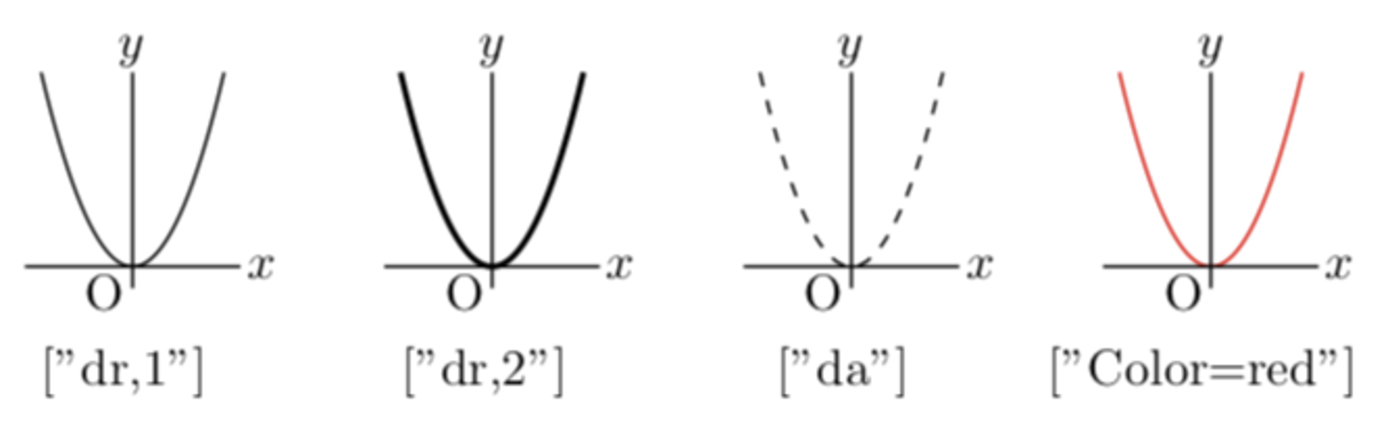
\includegraphics[bb=0.00 0.00 666.00 210.00,width=100mm]{fig/plotdatasample.pdf}}
\end{layer}

\begin{itemize}
\item
[課題]\monban 関数\verb|y=x^2|のグラフ\seteda{60}\\
\eda{線種("dr","da","do")を指定せよ}\\
\eda{"Color="を指定せよ}\\
\eda{Plotdataの行をコピペせよ}
\end{itemize}
%%%%%%%%%%%%

%%%%%%%%%%%%%%%%%%%%


\newslide{PDFの大きさの調整}

\vspace*{18mm}

\slidepage

\begin{layer}{100}{0}
\putnotese{95}{4}{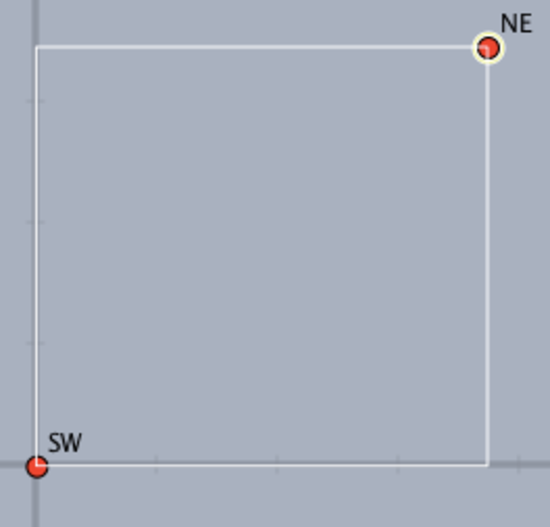
\includegraphics[bb=0.00 0.00 264.00 253.00,width=30mm]{fig/swne.pdf}}
\end{layer}

\begin{itemize}
\item
描画領域 SW,NEで囲まれる長方形\vspace{-2mm}
\item
描画領域に合ったPDFを出力したい.\vspace{6mm}
\item
手順\\
1.Ketinitの直後に Setparent(ファイル名)\\
 Cdyname()+"p" Cindy名に"p"をつける\\
2.Windispgの直前に Figpdf();\\
3.Figureの代わりにParentボタンを押す
\end{itemize}
\label{pageend}\mbox{}

\end{document}
